\documentclass{standalone}
\usepackage{tikz}
\usepackage{amsmath}
\usetikzlibrary{matrix}
\usetikzlibrary {shapes.geometric}
\usetikzlibrary {arrows.meta}
\begin{document}
    
        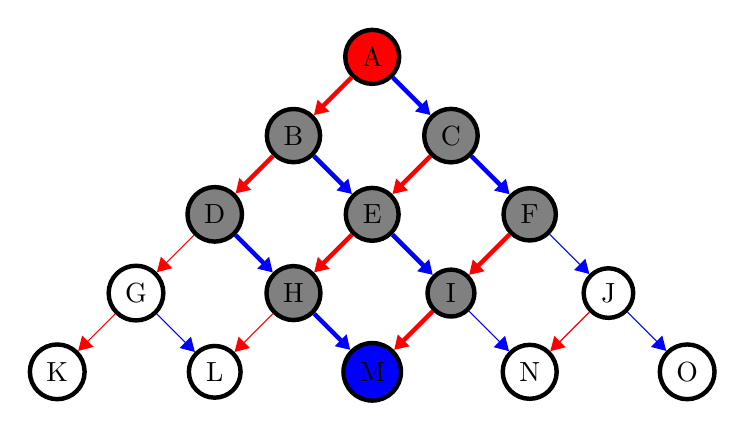
\begin{tikzpicture}[ultra thick]

            %\draw [help lines] (0,0) grid (10,10); 

            \path   (5,10)  node (a) [circle ,black,draw, fill = red] {A}
                    (4,9) node (b) [circle,draw,fill = gray] {B}
                    (6,9) node (c) [circle,draw,fill = gray] {C}
                    (3,8) node (d) [circle,draw,fill = gray] {D}
                    (5,8) node (e) [circle,draw,fill = gray] {E}
                    (7,8) node (f) [circle,draw,fill = gray] {F}
                    (2,7) node (g) [circle,draw] {G}
                    (4,7) node (h) [circle,draw,fill = gray] {H}
                    (6,7) node (i) [circle,draw,fill = gray] {I}
                    (8,7) node (j) [circle,draw] {J}
                    (1,6) node (k) [circle,draw] {K}
                    (3,6) node (l) [circle,draw] {L}
                    (5,6) node (m) [circle,draw,fill = blue] {M}
                    (7,6) node (n) [circle,draw] {N}
                    (9,6) node (o) [circle,draw] {O};
                
            \draw[ultra thick,arrows = -{Triangle[open,angle=60:2mm,fill = red]},red]  (node cs: name =a ) -> (node cs:name =b);
            \draw[ultra thick,arrows = -{Triangle[open,angle=60:2mm,fill = blue]},blue] (node cs: name =a ) -- (node cs:name =c);
            \draw[ultra thick,arrows = -{Triangle[open,angle=60:2mm,fill = red]},red] (node cs: name =b ) -- (node cs:name =d);
            \draw[ultra thick,arrows = -{Triangle[open,angle=60:2mm,fill = blue]},blue] (node cs: name =b ) -- (node cs:name =e);
            \draw[thin,arrows = -{Triangle[open,angle=60:2mm,fill = red]},red] (node cs: name =d ) -- (node cs:name =g);
            \draw[ultra thick,arrows = -{Triangle[open,angle=60:2mm,fill = red]},red] (node cs: name =c ) -- (node cs:name =e);
            \draw[ultra thick,arrows = -{Triangle[open,angle=60:2mm,fill = blue]},blue] (node cs: name =c ) -- (node cs:name =f);
            \draw[thin,arrows = -{Triangle[open,angle=60:2mm,fill = red]},red] (node cs: name =g ) -- (node cs:name =k);
            \draw[thin,arrows = -{Triangle[open,angle=60:2mm,fill = blue]},blue] (node cs: name =g ) -- (node cs:name =l);
            \draw[ultra thick,arrows = -{Triangle[open,angle=60:2mm,fill = blue]},blue] (node cs: name =d ) -- (node cs:name =h);
            \draw[thin,arrows = -{Triangle[open,angle=60:2mm,fill = red]},red] (node cs: name =h ) -- (node cs:name =l);
            \draw[ultra thick,arrows = -{Triangle[open,angle=60:2mm,fill = red]},red] (node cs: name =e ) -- (node cs:name =h);
            \draw[ultra thick,arrows = -{Triangle[open,angle=60:2mm,fill = blue]},blue] (node cs: name =h ) -- (node cs:name =m);
            \draw[ultra thick,arrows = -{Triangle[open,angle=60:2mm,fill = blue]},blue] (node cs: name =e ) -- (node cs:name =i);
            \draw[ultra thick,arrows = -{Triangle[open,angle=60:2mm,fill = red]},red] (node cs: name =i ) -- (node cs:name =m);
            \draw[thin,arrows = -{Triangle[open,angle=60:2mm,fill = blue]},blue] (node cs: name =i ) -- (node cs:name =n);
            \draw[ultra thick,arrows = -{Triangle[open,angle=60:2mm,fill = red]},red] (node cs: name =f ) -- (node cs:name =i);
            \draw[thin,arrows = -{Triangle[open,angle=60:2mm,fill = blue]},blue] (node cs: name =f ) -- (node cs:name =j);
            \draw[thin,arrows = -{Triangle[open,angle=60:2mm,fill = red]},red] (node cs: name =j ) -- (node cs:name =n);
            \draw[thin,arrows = -{Triangle[open,angle=60:2mm,fill = blue]},blue] (node cs: name =j ) -- (node cs:name =o);
        \end{tikzpicture}

\end{document}